\section{Konjunktur}
\textbf{Wachstum ist langfristig, Konjunktur kurzfristig.}

\begin{multicols}{2}
\subsection{Der negative Nachfrageschock}
\includegraphics[width=\linewidth]{images/negnach.png}
\vfill\null
\columnbreak
\subsection{Der kurzfristige positive Nachfrageschock}
\includegraphics[width=\linewidth]{images/posnachkurz.png}
\end{multicols}

\begin{multicols}{2}
\subsection{Der langfristige positive Nachfrageschock}
\includegraphics[width=\linewidth]{images/posnachlang.png}
\columnbreak
\subsection{Der negative Angebotsschock}
\includegraphics[width=\linewidth]{images/negangebot.png}
\end{multicols}

\begin{multicols}{2}
\subsection{Der positive Angebotsschock}
\includegraphics[width=\linewidth]{images/posangebot.png}
\columnbreak
\subsection{Konjunkturzyklen}
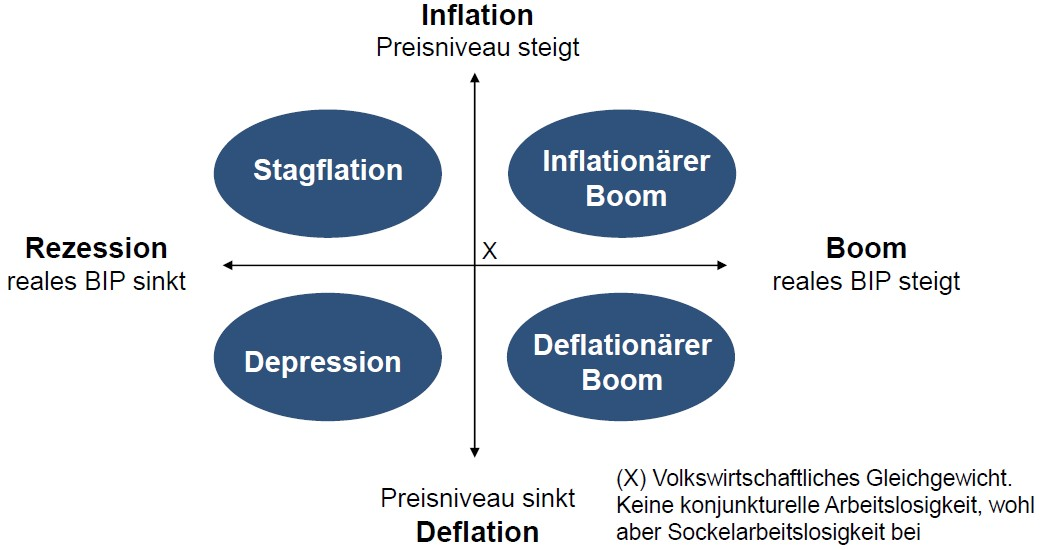
\includegraphics[width=\linewidth]{images/konjunkturzyklen.jpg}
\end{multicols}

\begin{minipage}{0.75\linewidth}
	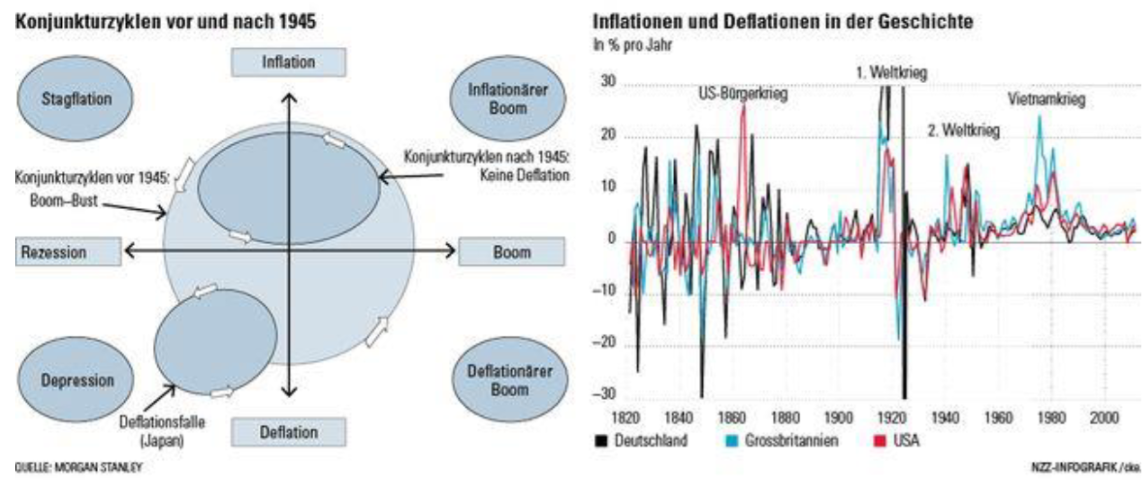
\includegraphics[width=\linewidth]{images/konjunkturzyklen2.png}
\end{minipage}%
\begin{minipage}{0.25\linewidth}
	Konjunkturzyklen nach 1945: Nationalbanken greifen ein, weil sie auf keinen Fall in eine Deflationsfalle geraten wollen.
\end{minipage}

\subsection{Das Phänomen der Arbeitslosigkeit}
\begin{multicols}{2}
\textbf{Konjunkturelle Arbeitslosigkeit (Y)}\\
Anzahl der Arbeitssuchenden ist grösser als die Anzahl der offenen Stellen (Ungleichgewichtsphänomen).\\
\textbf{Sockelarbeitslosigkeit (X)}\\
Anzahl der offenen Stellen ist gleich gross oder grösser als die Anzahl der Arbeitssuchenden. Dies kann zwei Gründe haben:
\begin{itemize}
	\item strukturelle Arbeitslosigkeit (Kap. \ref{sec:strukturelleArbeitslosigkeit})
	\item friktionelle Arbeitslosigkeit (Kap. \ref{sec:friktionelleArbeitslosigkeit})
\end{itemize}
\vspace{\baselineskip}
Y>X: falsche Ausbildung der Arbeitssuchenden
\vfill\null
\columnbreak
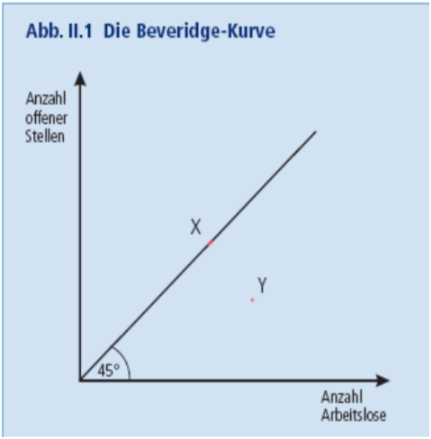
\includegraphics[width=0.8\linewidth]{images/arbeitslosigkeit.png}
\end{multicols}

\subsection{Bekämpfung der konjunkturellen Arbeitslosigkeit}
Die konjunkturelle Arbeitslosigkeit wird mit der Konjunkturpolitik bekämpft. Drei unterschiedliche Ansätze:\\
\textbf{1. "Nichts tun": Anpassung ohne aktive Konjunkturpolitik} $\rightarrow$ automatisches Wiederherstellen des langfristigen Gleichgewichts\\
\begin{itemize}
	\item kurzfristiger Effekt:
	\begin{itemize}
		\item reales BIP schrumpft, Preisniveau sinkt
		\item sinkende Nachfrage nach Arbeit
		\item (in "funktionierenden" Arbeitsmärkten) führt zu sinkenden Nominallöhnen
	\end{itemize}
	\item mittelfristiger Effekt:
	\begin{itemize}
		\item (falls Haushalte sinkende Nominallöhne akzeptieren) bedeutet tiefere Produktionskosten für Unternehmen
		\item höheres Angebot ($AA_K$ verschiebt sich nach rechts)
	\end{itemize}
	\item Ergebnis: gleiches reales BIP (Q1) bei tieferen Nominallöhnen, tieferem Preisniveau $\rightarrow$ gleiche Reallöhne
\end{itemize}
\includegraphics[width=0.5\linewidth]{images/nichts.png}%
\includegraphics[width=0.5\linewidth]{images/KorrekturKonjukArbeit}


\textbf{2. Aktive $"$keynesianische$"$ Konjunkturpolitik}\\
\begin{itemize}
	\item Märkte gehen von selbst, aber langsam wieder ins Gleichgewicht
	\item Positiver Nachfrageschock, ist vom Staat erreichbar durch:
	\begin{itemize}
		\item Fiskalpolitik:
		\begin{itemize}
			\item Stimulierung der Konsumnachfrage der Haushalte durch tiefere Steuern
			\item Erhöhung der Staatsausgaben (oft durch Verschuldung)
		\end{itemize}
		\item Geldpolitik (die Zentralbanken sind grundsätzlich unabhängig):
		\begin{itemize}
			\item Stimulierung der Investitionsnachfrage der Unternehmen durch tiefere Kreditzinsen (Erhöhung der Geldmenge)
			\item Erhöhung der Nettoexporte durch eine schwächere Währung (Erhöhung der Geldmenge)
		\end{itemize}
	\end{itemize}
\end{itemize}
\includegraphics[width=0.5\linewidth]{images/keyne.png}%
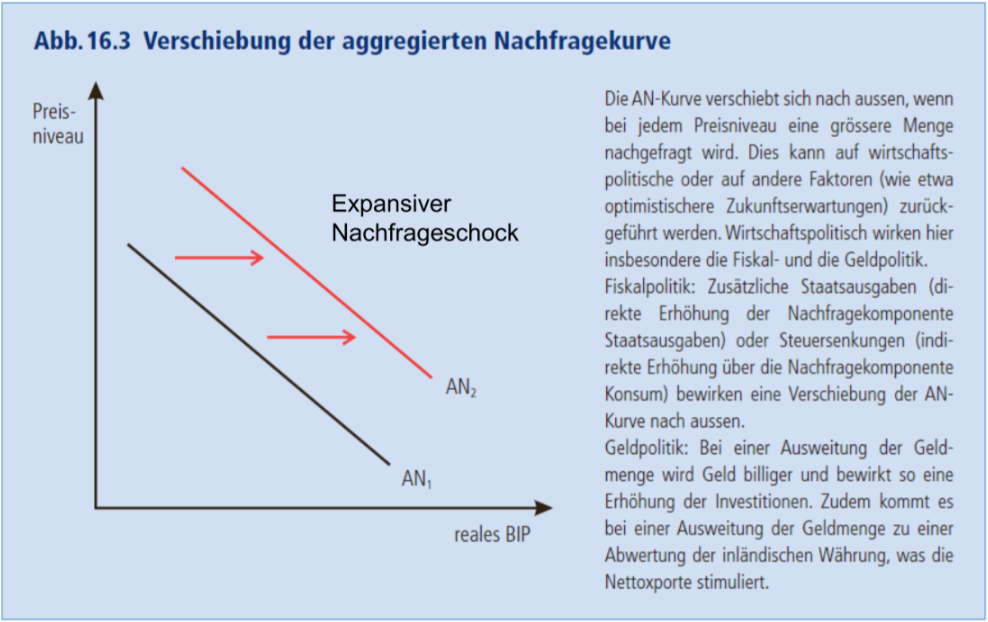
\includegraphics[width=0.5\linewidth]{images/keyne2.png}

\textbf{3. Stärkung der automatischen Stabilisatoren}\\
\begin{multicols}{2}
Staatliche Einnahmen und Ausgaben, die so ausgestaltet sind, dass bei einem Rückgang der gesamtwirtschaftlichen Nachfrage diese automatisch stimuliert wird.\\
\vspace{0.5cm}
automatische Stabilisatoren:
\begin{itemize}
	\item Schuldenbremse (Staatsausgaben = Staatseinnahmen)
	\item ALV
	\item Steuersystem
\end{itemize}
\vfill\null
\columnbreak
\includegraphics[width=\linewidth]{images/autostab.png}	
\end{multicols}
\clearpage

\subsection{Konjunkturpolitik}
\textbf{Problem der Wirkungsverzögerung}\\
\begin{itemize}
	\item Verzögerung in der Erkenntnis (mind. 6 Mt.)
	\item Verzögerung in der Implementierung (mind. 6 Mt.)
	\item Verzögerung in der Wirkung (~5 Jahre)
\end{itemize}
Die Konjunkturpolitik bekämpft oft erst dann die Rezession, während der wirtschaftliche Aufschwung bereits wieder voll eingesetzt hat.\\
\textbf{Grundsätzliche Problematik von politischen Anreizen}
\begin{itemize}
	\item Asymmetrische Handhabung (kein Eingriff gegen Hochkonjunktur)
	\item Permanente Budgetdefizite, welche zu einer laufenden Staatsverschuldung führen
	\item Konjunkturpolitik in Abhängigkeit von wahltaktischen Gründen (politische Konjunkturzyklen)
\end{itemize}
\textbf{Konjunkturpolitik in der Schweiz}\\
Die Schweizerische Bundesverfassung gibt dem Staat einen klaren konjunkturpolitischen Auftrag (Art. 100). Er \textbf{muss} Arbeitslosigkeit und Teuerung bekämpfen.\\
Auch die Nationalbank hat eine entsprechende Verpflichtung und muss in der Geldpolitik der Konjunktur Rechnung tragen (Nationalbankgesetz Art. 5).\\
In der Schweiz werden keynesianische Elemente in der Konjunkturpolitik kaum angewendet. Ein Grund dafür ist das föderalistische Staatssystem (Bund, Kantone und Gemeinden). Das Volk und die Kantone müssen dem Bund eine Macht übergeben, von sich aus kann der Bund nichts machen.\\
Die Schweizerische Konjunkturpolitik setzt vor allem auf die Anwendung von automatischen Stabilisatoren.\\
Auch die SNB hat sich in der Vergangenheit durch eine vorsichtige Anwendung der Geldpolitik im Rahmen der Konjunkturpolitik ausgezeichnet (diese Haltung hat sich allerdings in den letzten Jahren stark verändert).\\
\textbf{Schlechte Bilanz der Schweizer Konjunkturpolitik}\\
In den wenigen Fällen, in denen die Schweiz eine aktive $"$keynesianische$"$ Konjunkturpolitik betrieben hat, war die Bilanz in der Vergangenheit eher schlecht. Kein vergleichbares Land hat die Konjunkturschwankungen fiskalpolitisch in solchem Ausmass negativ verstärkt wie die Schweiz. Das zeigt u.a. eine aktuelle Studie der OECD.
\clearpage
\pagebreak

